\documentclass[a4paper,11pt,abstracton,hidelinks]{scrartcl}

\usepackage[margin=3cm]{geometry}
\usepackage{graphicx}
\usepackage[UKenglish]{babel}
\usepackage{csquotes}
\usepackage[style=authoryear-icomp,maxnames=1,uniquelist=false,backend=biber,doi=false,url=false]{biblatex}
\usepackage{float}
\usepackage[export]{adjustbox}
\usepackage[T1]{fontenc}
\usepackage{lmodern}
\usepackage[textsize=tiny]{todonotes}
\usepackage[labelsep=period,font=small,labelfont=bf,format=plain]{caption}
\captionsetup[table]{
  position=above,
  belowskip=10pt,
  aboveskip=0pt,
}
\usepackage[group-separator={,}]{siunitx}
\usepackage{booktabs}
\usepackage{pdflscape}
\usepackage{tablefootnote}
\usepackage{authblk}
\usepackage{threeparttable}
\usepackage{afterpage}
\usepackage{lineno}
\linenumbers
\usepackage{setspace}
\usepackage{hyperref}
\doublespacing

\newcommand{\beginsupplement}{%
  \setcounter{table}{0}
  \renewcommand{\thetable}{S\arabic{table}}%
  \setcounter{figure}{0}
  \renewcommand{\thefigure}{S\arabic{figure}}%
}

\usepackage{xspace}
\newcommand{\agam}{\textit{An. gambiae}\xspace}
\newcommand{\acol}{\textit{An. coluzzii}\xspace}
\newcommand{\vgsc}{\textit{Vgsc}\xspace}


\addbibresource{../refs.bib}


\title{Chapter 5. The molecular evolution and geographical spread of target-site resistance to pyrethroid insecticides among \textit{Anopheles gambiae} populations}


\author[1,2]{\small Alistair Miles}
\affil[1]{\footnotesize Big Data Institute, University of Oxford, Li Ka Shing Centre for Health Information and Discovery, Old Road Campus, Oxford OX3 7LF}
\affil[2]{\footnotesize Wellcome Sanger Institute, Hinxton, Cambridge CB10 1SA}


\begin{document}

\maketitle


\begin{abstract}


%%
TODO abstract
%%


\end{abstract}


%%%%%%%%%%%%%%%%%%%%%%%%%%%%%%%%%%%%%%%%%%%%%%%%%%%%%%%%%%%%%%%%%%%%%%%%%%%%%%%
%%%%%%%%%%%%%%%%%%%%%%%%%%%%%%%%%%%%%%%%%%%%%%%%%%%%%%%%%%%%%%%%%%%%%%%%%%%%%%%
\section*{Introduction}


%%%%%%%%%%%%%%%%%%%%%%%%%%%%%%%%%%%%%%%%%%%%%%%%%%%%%%%%%%%%%%%%%%%%%%%%%%%%%%%
\subsection*{Pyrethroids and their role in malaria control}


%% General introduction to pyrethroids and their role in malaria control.
%
Pyrethroids are a class of synthetic insecticides, based on a natural compound pyrethrin found in the flowers of pyrethrum (\textit{Chrysanthemum}) plants \autocite{Elliott1989}.
%
Pyrethroids suitable for commercial use in agriculture and public health were discovered in the 1970s, including permethrin \autocite{Elliott1973} and deltamethrin \autocite{Elliott1974}.
%
These compounds have a high toxicity to insects but relatively low toxicity to mammals, and are photostable but do not accumulate to contaminate the environment.
%
Pyrethroids were approved for use in public health by the WHO pesticide evaluation scheme (WHOPES) in @@year @@cite.
%
Initially they were proposed for using in space and residual spraying, however it was also found that they could be impregnated into bed-nets @@cite.
%
Several landmark clinical trials during the 1980s showed that the use of pyrethroid-treated bed-nets caused a significant reduction in malaria @@cite.
%
Advances in net manufacturing subsequently allowed the development of long-lasting insecticidal nets (LLINs) which retained insecticidal activity for up to 3 years without retreatment @@cite.
%
Pyrethroid LLINs became the cornerstone of efforts to scale up malaria control interventions in Africa, led by the Roll Back Malaria Consortium, beginning in 1998 @@cite.
%
Those efforts have continued to expand, with @@200 million pyrethroid LLINs distributed for free in Africa in @@year, by the Global Fund and other international partner organisations @@cite.
%
The widespread use of pyrethroid LLINs has had a major impact on malaria burden, with models based on data aggregated from studies in Africa between 2000 and 2015 estimating that LLINs account for @@what fraction of the reduction in malaria cases @@cite.
%%


%%%%%%%%%%%%%%%%%%%%%%%%%%%%%%%%%%%%%%%%%%%%%%%%%%%%%%%%%%%%%%%%%%%%%%%%%%%%%%%
\subsection*{Pyrethroid resistance in malaria vectors}


%% Brief history of pyrethroid resistance in malaria vectors.
%
The first reports of resistance to pyrethroids among malaria vector populations were made during the 1980s.
%
For example, in @@examples of early resistance reports.
%
These reports coincided with the widespread adoption of pyrethroids in agriculture, and with the increased availability of personal and household protection products using pyrethroids @@verify @@cite.
%
As LLIN distribution was scaled up in Africa from 1998 onwards, malaria control programmes were encouraged to regularly test vector populations for evidence of pyrethroid resistance, via standardised bioassays @@cite.
%
As those data have accumulated, it is clear that the geographical extent of pyrethroid resistance among malaria vector populations has substantially increased in the last 20 years @@cite.
%
For example, @@example of areas where prevalence of resistance has increased.
%
Pyrethroids remain an essential component of all LLIN products currently approved for public health use, and thus resistance to pyrethroids is viewed as a serious challenge to the efficacy of future malaria control efforts @@cite.
%%


%%%%%%%%%%%%%%%%%%%%%%%%%%%%%%%%%%%%%%%%%%%%%%%%%%%%%%%%%%%%%%%%%%%%%%%%%%%%%%%
\subsection*{The pyrethroid mode of action}


%% Introduction to the VGSC protein and the pyrethroid mode of action.
%
Pyrethroids disrupt the insect nervous system, causing paralysis ("knock-down") and then death @@cite.
%
Pyrethroid molecules interact with the voltage-gated sodium channel (VGSC), an essential membrane protein which propagates nerve impulses via action potentials @@cite.
%
The VGSC protein sequence of \textit{Anopheles gambiae}, the major vector of malaria in Africa, comprises @@N amino acids and has a high degree of homology with sequences from other insect species @@cite.
%
In all insects the protein comprises four repeated subunits, each of which has 6 transmembrane domains @@check @@cite.
%
Between each of the four subunits are internal linker segments @@TODO check @@TODO ref.
%
Within each sububit there are smaller linker segments joining the transmembrane domains, which may be internal or external to the cell @@cite.
%
The transmembrane segments together form a pore or channel, and @@describe the gating components which allow the firing and then restoration of polarisation@@.
%
In the presence of a pyrethroid, VGSC proteins @@describe physiological effect@@, as shown via oocyte experiments @@cite, suggesting @@what the gating function is disrupted and resting potential cannot be restored@@.
%%


%%%%%%%%%%%%%%%%%%%%%%%%%%%%%%%%%%%%%%%%%%%%%%%%%%%%%%%%%%%%%%%%%%%%%%%%%%%%%%%
\subsection*{Molecular biology of pyrethroid target-site resistance in \agam}


%% Brief review of molecular biology of VGSC pyrethroid resistance in An. gambiae.
%
In \agam the molecular biology of resistance has appeared to be relatively straightforward according to previous studies.
%
A \texttt{L995F} @@ref codon numbering@@ substitution was first found @@history of L995F@@.
%
@@resistance phenotype of L995F@@
%
A second substitution in the same codon, L995S, was subsequently found @@history of L995S@.
%
@@resistance phenotype of L995S@@
%
Initially \texttt{L995F} was found only in populations from West African countries, and \texttt{L995S} only in East Africa.
%
Because of the classical ``knock-down resistance'' phenotype, and their initial geographical distribution, the two substitutions \texttt{L995F} and \texttt{L995S} are sometimes referred to as \textit{kdr-West} and \textit{kdr-East} respectively.
%
However, more recent studies have found a broader geographical distribution, e.g., @@studies with kdr-west in east and/or vice versa@@.
%
A third substitution, N1570Y, was found in @@origin, apparently as a secondary mutation occurring only on haplotypes carrying \texttt{L995F} @@cite.
%
In vitro studies subsequently showed that the combination of L995+N1570Y had significantly higher pyrethroid resistance @@details @@cite, thus it appears that there is ongoing molecular evolution.
%%


%%%%%%%%%%%%%%%%%%%%%%%%%%%%%%%%%%%%%%%%%%%%%%%%%%%%%%%%%%%%%%%%%%%%%%%%%%%%%%%
\subsection*{Molecular biology of pyrethroid target-site resistance in other insects}


%% Brief review of molecular biology of VGSC pyrethroid resistance in other insects.
%
In other insects the molecular biology of VGSC-mediated pyrethroid resistance appears to be more varied and complex.
%
For example, @@summarise house fly@@.
%
In comparison, among mosquitoes of the \textit{Aedes} genus, @@summarise aedes@@.
%
Among the VGSC substitutions found across all insects, more than @@N have been shown to functionally affect pyrethroid resistance in vitro, and a further @@N have been found to be associated with resistance in vivo @@cite.
%
An interesting feature of these substitions are the protein locations in which they occur.
%
In silico molecular modelling studies have predicted that there are two independent pyrethroid binding sites within the VGSC channel, referred to as @@names @@cite.
%
Several of the primary resistance substitutions are found within one of these two predicted binding sites, including codon \texttt{995} where \textit{kdr} mutations are found in \agam, and @@other codons in other species@@.
%
Resistance mutations within the pyrethroid binding sites make obvious sense, as they can reasonably be assumed to alter the conformation or shape of the binding site in some way, and thus disrupt the interaction with pyrethroid molecules @@cite.
%
However, many other mutations shown to have a resistance phenotype do not occur in either binding site or even within a transmembrane domain, with many occurring in internal or external linker domains.
%
For example, \texttt{N1570Y} occurs in the internal linker between @@segments @@cite.
%
Modelling work on \texttt{N1570Y} has suggested that this might have an allosteric effect on the conformation of the pyrethroid binding site @@cite.
%
However, it has also been suggested that linker segments play a role in the dynamics and modulation of gating kinetics, and so modifications in these segments may play a more subtle and indirect role in disrupting or compensating for the pyrethroid mode of action @@cite.
%
Several substitutions, such as N1570Y, only occur in association with another substitution, indicating important epistatic interactions between different sites in the protein sequence.
%
Studies in \agam mosquitoes have to date mostly focused on partial sequencing of a limited number of exons, and thus the full coding sequence has not been thoroughly surveyed across multiple populations.
%%


%%%%%%%%%%%%%%%%%%%%%%%%%%%%%%%%%%%%%%%%%%%%%%%%%%%%%%%%%%%%%%%%%%%%%%%%%%%%%%%
\subsection*{Geographical origins of pyrethroid target-site resistance in \agam}


%% Open questions regarding the geographical and etiological origins of VGSC pyrethroid resistance in An. gambiae.
%
Although there is little doubt that the prevalence of pyrethroid resistance among \agam populations has increased substantially in recent years, there remain a number of open questions regarding the underlying factors and processes driving this increase in prevalence.
%
The \texttt{L995F} allele is now found widely throughout West and Central Africa, but it is not known whether this apparent spread is due to gene flow alone, or whether the allele arose from multiple geographical origins.
%
@@TODO what did the Pinto paper say about kdr origins? @@TODO any other data on kdr origins, e.g., Lynd paper?
%
@@TODO spread of \texttt{L995F} between gambiae and coluzzii, Clarkson and other paper.
%
Similarly, the \texttt{L995S} allele is now at high frequency throughout East and Central Africa, but its geographical origins and patterns of gene flow are unknown.
%
It would be valuable to know whether the occurrence of any given insecticide resistance allele in two geographically distinct mosquito populations can be traced back to a recent common ancestor, and therefore that the allele has arrived in both populations via contemporary gene flow from a common geographical origin.
%
This information would enable us to unravel the history of an insecticide resistance outbreak, and undertake a systematic analysis of the factors driving its spread.
%
This kind of inference has previously been difficult for \vgsc resistance alleles, however, due to the limited resolution of the available sequence data.
%%


%%%%%%%%%%%%%%%%%%%%%%%%%%%%%%%%%%%%%%%%%%%%%%%%%%%%%%%%%%%%%%%%%%%%%%%%%%%%%%%
\subsection*{Pyrethroid resistance as a model system for studying evolutionary dynamics}


%% Broaden out to other examples of ongoing selective sweeps.
%
As well as representing a pressing public health emergency, pyrethroid resistance in \agam represents a phenomenon of fundamental biological interest, because it provides an opportunity to study an ongoing evolutionary event in nature, occuring on an observable time scale.
%
Furthermore, this evolutionary event is occurring in a complex of species with incomplete reproductive isolation, whose broad geographical range spans an entire continent and a variety of ecological settings.
%
Further complexity is added by the fact that this event is being driven by strong but patchy and varying selective pressures.
%
There are geographical and temporal heterogeneities in both agricultural insecticide usage and public health vector control interventions, which are themselves evolving as new LLIN and IRS products become available and are transitioned into large scale public health campaigns.
%
As this event unfolds, it provides an opportunity to observe the evolution of the VGSC protein sequence, which happens to be a fundamental protein with otherwise high levels of conservation across multiple phyla.
%
It also provides a unique window into population dynamic processes within mosquito populations, because it reveals connectivities between populations and species, as selective advantage drives new adaptations rapidly across the landscape.
%
@@TODO compare with other examples of ongoing evolution. crop pests? parasites under drug pressure? adaptations to industrialisation/urbanisation?
%%


%%%%%%%%%%%%%%%%%%%%%%%%%%%%%%%%%%%%%%%%%%%%%%%%%%%%%%%%%%%%%%%%%%%%%%%%%%%%%%%
\subsection*{Scope of this chapter}


%% paragraph segue to scope of this paper
%
In this chapter I analyse data from phase 1 of the \textit{Anopheles gambiae} 1000 Genomes Project to investigate the molecular evolution and geographical spread of target-site resistance to pyrethroids.
%
I report on the discovery of a number of mutations at appreciable frequency that alter the protein-coding sequence of the gene, and which therefore may have some phenotypic effect.
%
I also investigate the linkage between these mutations, to determine whether some alleles occur in association with others, and thus whether there may be any epistatic interactions between them.
%
I then use data on non-coding mutations both within the gene introns and in the flanking intergenic sequences to investigate the genetic backgrounds (haplotypes) on which insecticide resistance alleles occur.
%
I describe a number of complementary analyses of the genetic relatedness between haplotypes, and use those analyses to make inferences about gene flow events between populations from different geographical locations and species.
%%


%%%%%%%%%%%%%%%%%%%%%%%%%%%%%%%%%%%%%%%%%%%%%%%%%%%%%%%%%%%%%%%%%%%%%%%%%%%%%%%
%%%%%%%%%%%%%%%%%%%%%%%%%%%%%%%%%%%%%%%%%%%%%%%%%%%%%%%%%%%%%%%%%%%%%%%%%%%%%%%
\section*{Results}


%%%%%%%%%%%%%%%%%%%%%%%%%%%%%%%%%%%%%%%%%%%%%%%%%%%%%%%%%%%%%%%%%%%%%%%%%%%%%%%
\subsection*{Non-synonymous variation}


%% Discovery of non-synonymous variation in Vgsc from Ag1000G phase 1. Analysis of genome accessibility within Vgsc.
%
I extracted data on variation within the \vgsc gene from the \textit{Anopheles gambiae} 1000 Genomes Project phase 1 AR3 data release, and annotated each variant according to its effect on the protein coding sequence (Methods).
%
Within the gene a total of @@N non-synonymous polymorphisms were found.
%
Of these, @@N passed all of the genome-wide quality filters previously applied, and @@N failed.
%
One of the SNPs failing quality filters included the @@N1570Y variant, previously found to be an important modifier of the pyrethroid resistance phenotype (@@cite).
%
Genome-wide SNP filters were generally conservative, erring on the side of reducing the false discovery rate at the expense of sensitivity.
%
Because any non-synonymous variant in the \vgsc gene could potentially cause an important phenotypic effect, I undertook a detailed manual examination of genome accessibility within all coding regions within the gene (Supplementary Figure \ref{fig:accessibility}).
%
In general, SNPs that failed quality filters were close to the thresholds set, and there was no substantial evidence for structural variation, alignment ambiguity or other alignment issues which could cause false discoveries.
%
All non-synonymous variants discovered in the gene were therefore included in subsequent analyses.
%%


%% Calculation of population allele frequencies; filtering of variants by frequency.
%
I then computed the frequency of each non-synonymous allele within each of nine populations defined by species and country of origin.
%
If an allele has a resistance phenotype and has been under positive selection, it will occur at some appreciable frequency within one or more populations.
%
I therefore filtered the variants to retain only those that occurred at a population frequency above 5\%.
%
This resulted in a set of @@N variant alleles (Table \ref{table:variants_missense}).
%
Two variant alleles were found at position @@N, and two variant alleles were found at position @@M.
%
The @@WHICH allele did not occur at 5\% frequency in any population, however the other variant allele at the same site did, and both alleles were included in @@TABLE as the occurrence of two alleles at the same site could indicate an important site within the protein.
%
Another feature of important sites within the protein is the occurrence of multiple substitutions at the same amino acid site.
%
Codon \texttt{995} provides the canonical example, with the \texttt{L995F} and \texttt{L995S} polymorphisms occurring at adjacent nucleotides but affecting the same codon.
%
@N other similar examples were found.
%
@@Other examples of two SNPs in the same codon.
%%


%% Table - Non-synonymous SNPs.
%
\afterpage{%
%\clearpage
% N.B., for some reason using \newgeometry causes page number to get dropped from the subsequent page, so disable for now - not needed if using \footnotesize.
\newgeometry{margin=2cm}
\begin{landscape}
\thispagestyle{empty}
\begin{table}[h]
  \scriptsize
  \centering
  \begin{threeparttable}

  \caption{
%
\textbf{Non-synonymous nucleotide variation in the voltage-gated sodium channel gene}.
%
AO=Angola; BF=Burkina Faso; GN=Guinea; CM=Cameroon; GA=Gabon; UG=Uganda; KE=Kenya; GW=Guinea-Bissau; \textit{Ac}=\acol; \textit{Ag}=\agam.
%
Species status of specimens from Kenya and Guinea-Bissau is uncertain @@cite.
%
All variants are at 5\% frequency or above in one or more of the 9 Ag1000G phase 1 populations, with the exception of \texttt{2,400,071 G>T} which is only found in the CM\emph{Ag} population at 0.4\% frequency but is included because another mutation (\texttt{2,400,071 G>A}) is found at the same position causing the same amino acid substitution (\texttt{M490I}); and \texttt{2,431,019 T>C} (\texttt{F1920S}) which is at 4\% frequency in GA\emph{Ag} but also found in CM\emph{Ag} and linked to \texttt{L995F}.
}

  \label{table:variants_missense}

  
\begin{tabular}{llllrrrrrrrrr}
\toprule
\multicolumn{4}{c}{Variant} &
\multicolumn{9}{c}{Population allele frequency (\%)}\\
\cmidrule(r){1-4}
\cmidrule(r){5-13}
Position\tnote{1} & 
\emph{Ag}\tnote{2} & 
\emph{Md}\tnote{3} &
Domain\tnote{4} &
AO\emph{Ac} & 
BF\emph{Ac} & 
GN\emph{Ag} & 
BF\emph{Ag} & 
CM\emph{Ag} & 
GA\emph{Ag} & 
UG\emph{Ag} & 
KE & 
GW\\
\midrule

\texttt{2,390,177 G>A} & \texttt{R254K} & \texttt{R261} & \texttt{IL45} & 0 & 0 & 0 & 0 & 32 & 21 & 0 & 0 & 0 \\

\texttt{2,391,228 G>C} & \texttt{V402L} & \texttt{V410} & \texttt{IS6} & 0 & 7 & 0 & 0 & 0 & 0 & 0 & 0 & 0 \\

\texttt{2,391,228 G>T} & \texttt{V402L} & \texttt{V410} & \texttt{IS6} & 0 & 7 & 0 & 0 & 0 & 0 & 0 & 0 & 0 \\

\texttt{2,399,997 G>C} & \texttt{D466H} & \texttt{-} & \texttt{LI/II} & 0 & 0 & 0 & 0 & 7 & 0 & 0 & 0 & 0 \\

\texttt{2,400,071 G>A} & \texttt{M490I} & \texttt{M508} & \texttt{LI/II} & 0 & 0 & 0 & 0 & 0 & 0 & 0 & 18 & 0 \\

\texttt{2,400,071 G>T} & \texttt{M490I} & \texttt{M508} & \texttt{LI/II} & 0 & 0 & 0 & 0 & 0 & 0 & 0 & 0 & 0 \\

\texttt{2,416,980 C>T} & \texttt{T791M} & \texttt{T810} & \texttt{IIS1} & 0 & 1 & 13 & 14 & 0 & 0 & 0 & 0 & 0 \\

\texttt{2,422,651 T>C} & \texttt{L995S} & \texttt{L1014} & \texttt{IIS6} & 0 & 0 & 0 & 0 & 15 & 64 & 100 & 76 & 0 \\

\texttt{2,422,652 A>T} & \texttt{L995F} & \texttt{L1014} & \texttt{IIS6} & 86 & 85 & 100 & 100 & 53 & 36 & 0 & 0 & 0 \\

\texttt{2,424,384 C>T} & \texttt{A1125V} & \texttt{K1133} & \texttt{LII/III} & 9 & 0 & 0 & 0 & 0 & 0 & 0 & 0 & 0 \\

\texttt{2,425,077 G>A} & \texttt{V1254I} & \texttt{I1262} & \texttt{LII/III} & 0 & 0 & 0 & 0 & 0 & 0 & 0 & 0 & 5 \\

\texttt{2,429,617 T>C} & \texttt{I1527T} & \texttt{I1532} & \texttt{IIIS6} & 0 & 14 & 0 & 0 & 0 & 0 & 0 & 0 & 0 \\

\texttt{2,429,745 A>T}* & \texttt{N1570Y} & \texttt{N1575} & \texttt{LIII/IV} & 0 & 26 & 10 & 22 & 6 & 0 & 0 & 0 & 0 \\

\texttt{2,429,897 A>G} & \texttt{E1597G} & \texttt{E1602} & \texttt{LIII/IV} & 0 & 0 & 6 & 4 & 0 & 0 & 0 & 0 & 0 \\

\texttt{2,429,915 A>C} & \texttt{K1603T} & \texttt{K1608} & \texttt{IVS1} & 0 & 5 & 0 & 0 & 0 & 0 & 0 & 0 & 0 \\

\texttt{2,430,424 G>T} & \texttt{A1746S} & \texttt{A1751} & \texttt{IVS5} & 0 & 0 & 11 & 13 & 0 & 0 & 0 & 0 & 0 \\

\texttt{2,430,817 G>A} & \texttt{V1853I} & \texttt{V1858} & \texttt{COOH} & 0 & 0 & 8 & 5 & 0 & 0 & 0 & 0 & 0 \\

\texttt{2,430,863 T>C} & \texttt{I1868T} & \texttt{I1873} & \texttt{COOH} & 0 & 0 & 18 & 25 & 0 & 0 & 0 & 0 & 0 \\

\texttt{2,430,880 C>T} & \texttt{P1874S} & \texttt{P1879} & \texttt{COOH} & 0 & 21 & 0 & 0 & 0 & 0 & 0 & 0 & 0 \\

\texttt{2,430,881 C>T} & \texttt{P1874L} & \texttt{P1879} & \texttt{COOH} & 0 & 7 & 45 & 26 & 0 & 0 & 0 & 0 & 0 \\

\texttt{2,431,019 T>C} & \texttt{F1920S} & \texttt{Y1925} & \texttt{COOH} & 0 & 0 & 0 & 0 & 1 & 4 & 0 & 0 & 0 \\

\texttt{2,431,061 C>T} & \texttt{A1934V} & \texttt{A1939} & \texttt{COOH} & 0 & 12 & 0 & 0 & 0 & 0 & 0 & 0 & 0 \\

\texttt{2,431,079 T>C} & \texttt{I1940T} & \texttt{I1945} & \texttt{COOH} & 0 & 4 & 0 & 0 & 7 & 0 & 0 & 0 & 0 \\

\bottomrule
\end{tabular}


  \begin{tablenotes}
    \footnotesize

    \item[1] Position relative to the AgamP3 reference sequence, chromosome arm 2L. Variants marked with an asterisk (*) failed conservative variant filters applied genome-wide in the Ag1000G phase 1 AR3 callset, but appeared sound on manual inspection of read alignments.

    \item[2] Codon numbering according to \emph{Anopheles gambiae} transcript AGAP004707-RA in geneset AgamP4.4.

    \item[3] Codon numbering according to \emph{Musca domestica} EMBL accession X96668 @@cite.

    \item[4] Location of the variant within the protein structure. Transmembrane segments are named according to domain number (in Roman numerals) followed by `S' then the number of the segment; e.g., `IIS6' means domain two, transmembrane segment six. Internal linkers between segments within the same domain are named according to domain (in Roman numerals) followed by `L' then the numbers of the linked segments; e.g., `IL45' means domain one, linker between transmembrane segments four and five. Internal linkers between domains are named `L' followed by the linked domains; e.g., `LI/II' means the linker between domains one and two. `COOH' means the internal carboxyl tail.

  \end{tablenotes}

  \end{threeparttable}

\end{table}
\end{landscape}
\restoregeometry
} % end afterpage
%% end Table 1


%% Transcript variation.
%
The \vgsc gene is known to undergo splicing variation in multiple insect species, and this is believe to be an important factor enabling insects to achieve some phenotypic variation @@CITE.
%
For \agam, three separate transcripts were reported in the official gene annotations from vectorbase, which derived from RNA sequencing of @@PEST?
%
However, the canonical study of the \vgsc gene in \agam is @@CITE Davies@@, where significantly greater splice variation was reported.
%
A difficulty of the Davies data is that there are no complete transcript sequences, only separate sequences from the first and second halves of the transcript.
%
To allow for all possibilities, I constructed a set of alternative transcripts from all possible combinations of the first and second half sequences from Davies et al. @@cite (Supplementary Figure \ref{fig:transcripts}).
%
I then reannotated all variants discovered within the \vgsc gene with each of these alternative transcripts, to determine whether any important non-synonymous variants had occurred within an exon segment not present in the canonical gene model (@@AGAP...-RA).
%
@@N non-synonymous variants were found in exon segments not found in AGAP...-RA, but none of these occurred at above @@X\% frequency in any population, and therefore were not considered in further analyses.
%%


%%%%%%%%%%%%%%%%%%%%%%%%%%%%%%%%%%%%%%%%%%%%%%%%%%%%%%%%%%%%%%%%%%%%%%%%%%%%%%%
\subsection*{Epistatic interactions}


%% Introduction to LD analysis, what types of association are we looking for, how do we measure it.
%
As mentioned earlier, a number of epistatic interactions between non-synomous mutations within the \vgsc gene have previously been reported, both in \agam and in other insects.
%
Of most immediate relevance to \agam is the \texttt{N1570Y} mutation, which has been found in subordinate association with the \texttt{L995F} mutation @@CITE, and shown to increase the pyrethroid resistance phenotype by up to an order of magnitude @@CITE.
%
By ``subordinate association'' here I mean that \texttt{N1570Y} is only ever found on haplotypes also carrying \texttt{L995F}.
%
This type of association can be measured as almost complete linkage disequilibrium between the two alleles ($D' \simeq 1$), with the primary allele always occurring at higher population frequency than the subordinate allele.
%
This pattern of association is consistent with the primary allele acting as a driver, providing a resistance phenotype and experiencing positive selection by itself, and the subordinate allele acting either to enhance the resistance phenotype or to compensate for some moderate deleterious effect of the primary allele on the normal function of the protein.
%
Another type of association is illustrated by pairs of alleles which are only ever found together, which I refer to here as ``complete association''.
%
Examples of complete associations include @@TODO examples.
%
Complete association can be measured as almost complete linkage disequilibrium, with the two alleles at equal frequencies within each population in which they occur.
%
Complete association indicates a strong epistatic interaction between two alleles, where either alone is deleterious regardless of the presence or absence of insecticide selective pressure, but both alleles occurring together provide some resistance phenotype and are positively selected.
%%


%%
%
To investigate epistatic interactions within the present dataset, I calculated the $D'$ linkage disequilibrium statistic (@@CITE) between all pairs of non-synonymous variant alleles (Methods).
%
The haplotype data from Ag1000G phase 1 only included biallelic SNPs passing all quality filters, and thus did not include \texttt{N1570Y} due to failing filters or multiallelic SNPs at positions \texttt{2L:2391228} and \texttt{2L:2400071}.
%
To incorporate these alleles into the analysis, I phased these alleles onto the biallelic haplotype scaffold (Methods).
%
The LD values are shown together with overall allele frequencies within the Ag1000G phase 1 cohort in Figure \ref{fig:ld}.
%%


%% Figure - Pairwise LD.
%
\begin{figure}[!t]

  \centering

  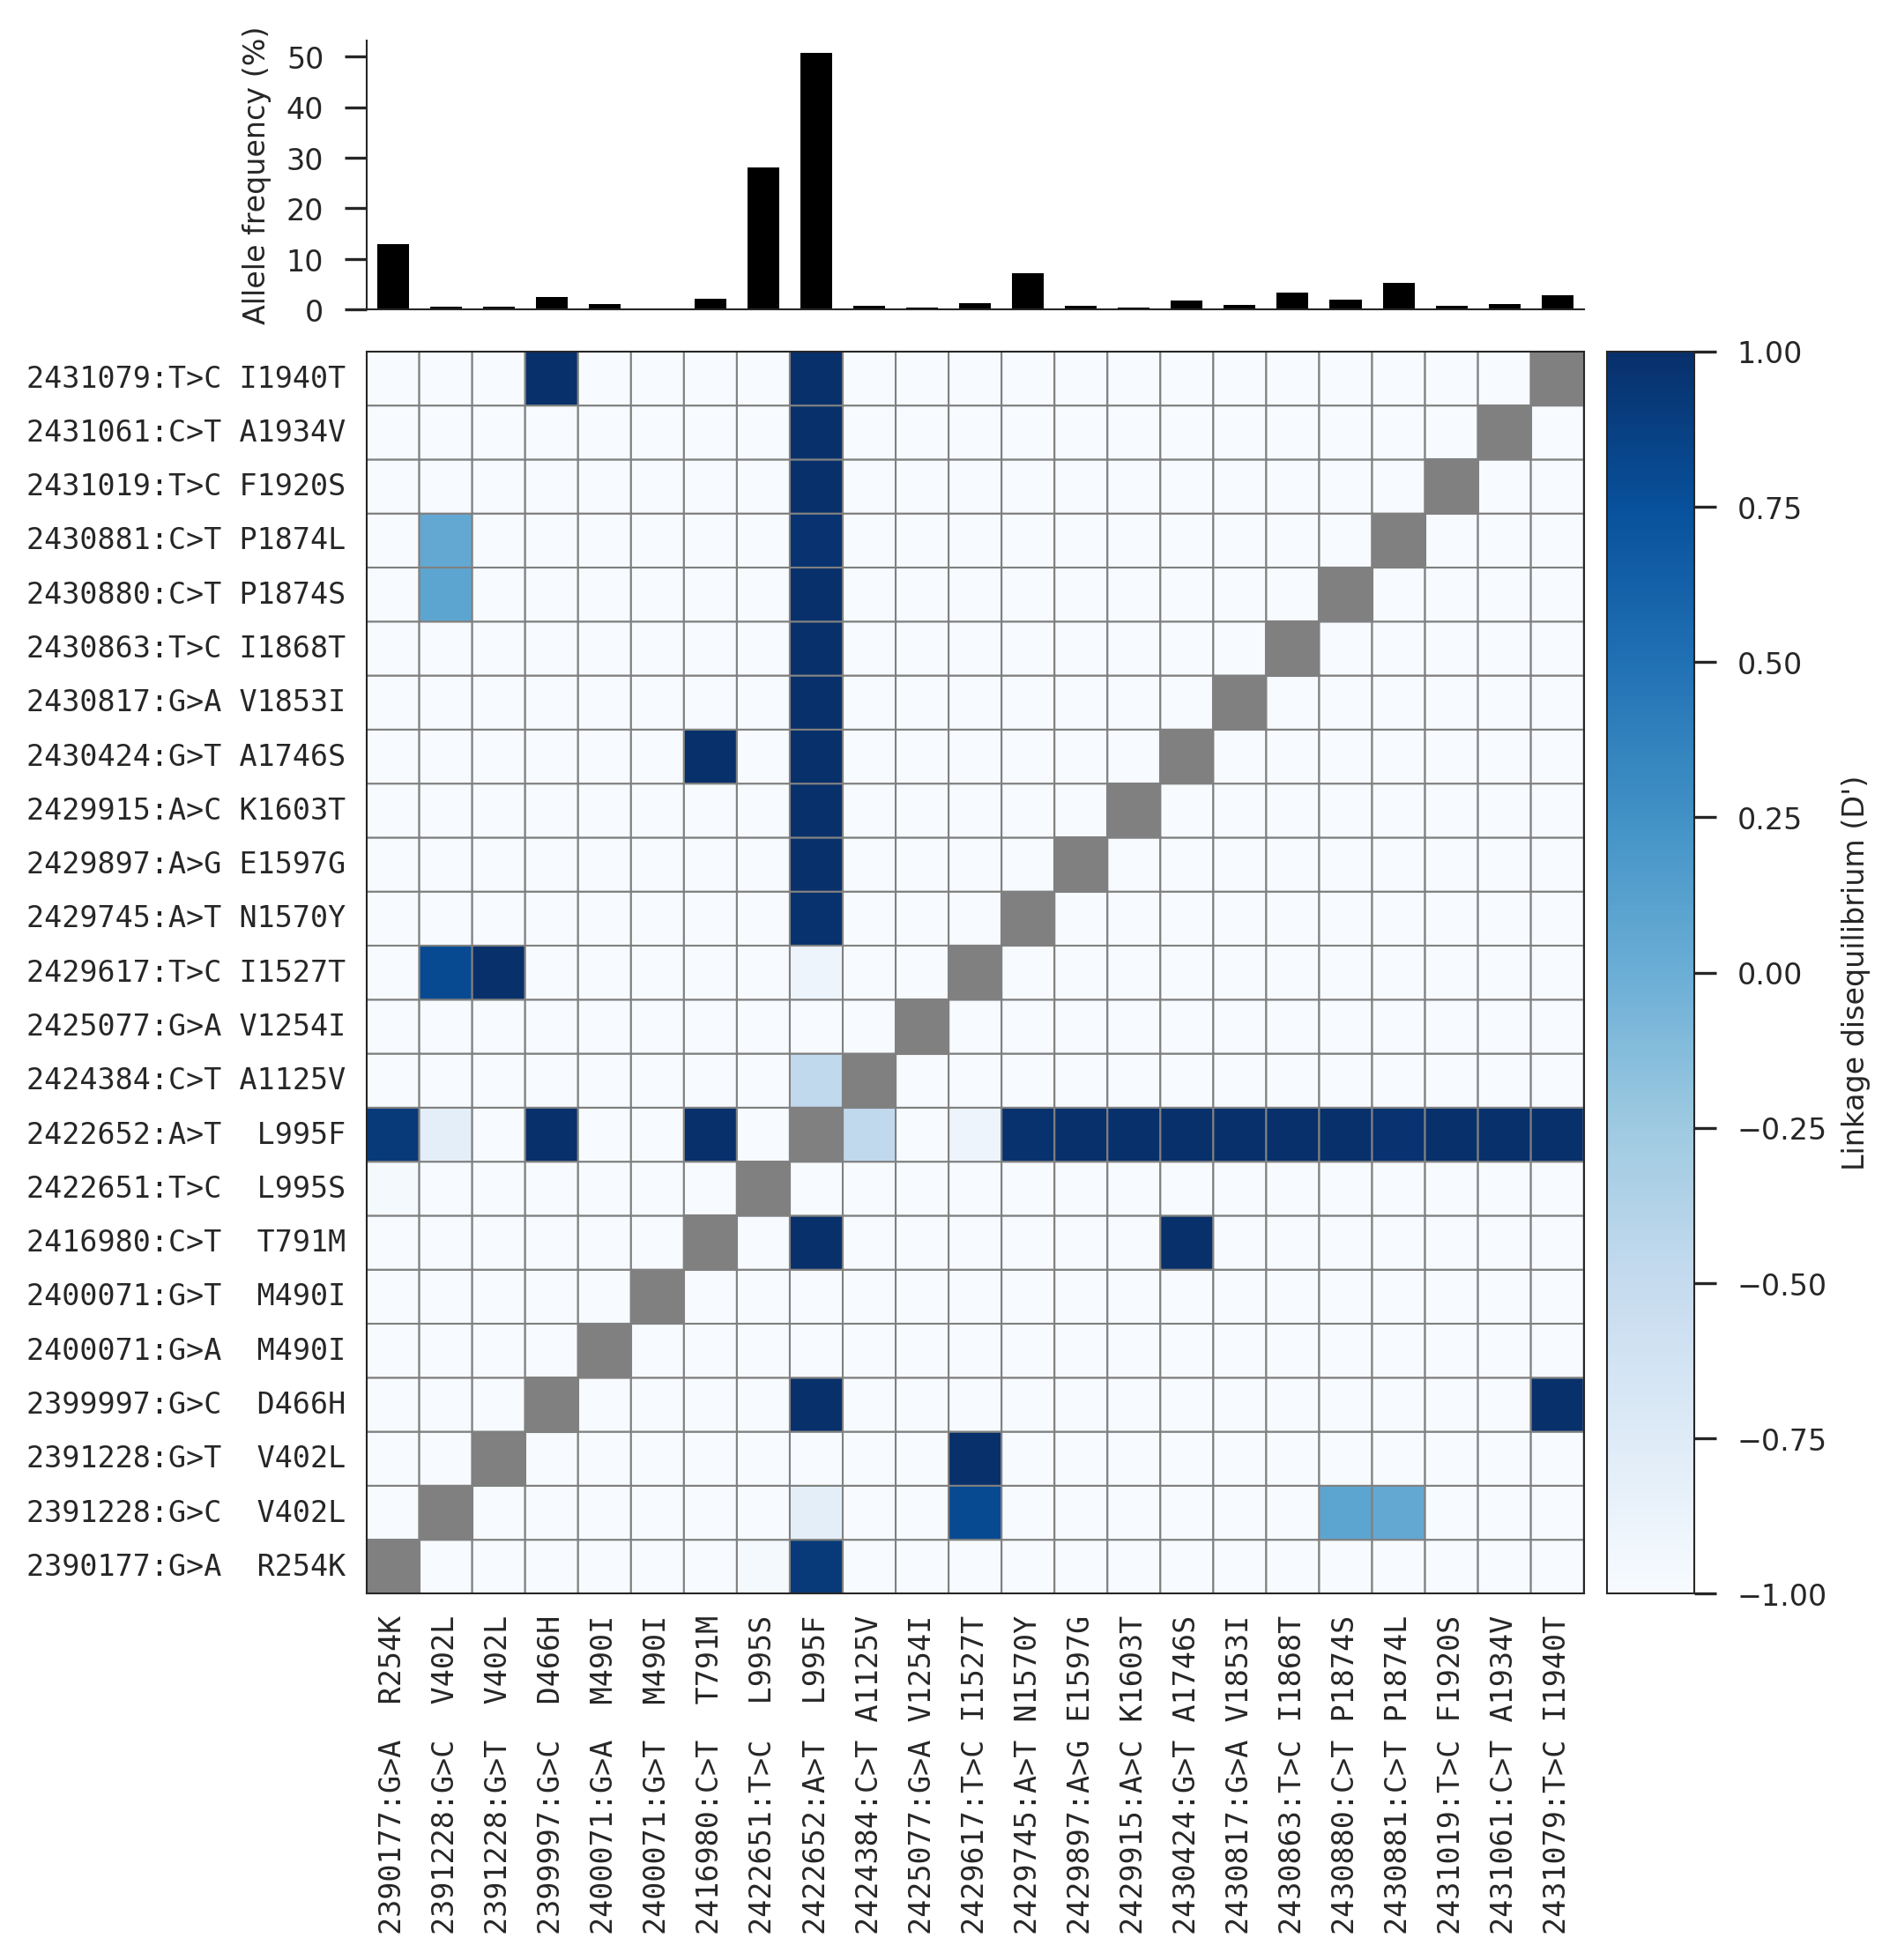
\includegraphics[width=\linewidth]{artwork/fig_ld.png}

  \caption{\textbf{Linkage disequilibrium ($D'$) between non-synonymous variants}. A value of 1 indicates that two alleles are in perfect linkage, meaning that one of the alleles is only ever found in combination with the other. Conversely, a value of -1 indicates that two alleles are never found in combination with each other. The bar plot at the top shows the frequency of each allele within the Ag1000G phase 1 cohort. See Table \ref{table:variants_missense} for population allele frequencies.}

  \label{fig:ld}

\end{figure}
%%


%% describe patterns of LD on kdr alleles
Fourteen high frequency non-synonymous variants occurred in strong LD ($D' > @@$) with \texttt{L995F} and always in subordinate association (Figure \ref{fig:ld}). 
%
These included \texttt{N1570Y}, known to modify the pyrethroid resistance phenotype @@cite and previously found in @@country @@cite.
%
These also included two variants in codon \texttt{1874}.
%
Substitutions in the orthologous codon have been observed in a colony of the diamond back moth \textit{Plutella xylostella} with a pyrethroid resistance phenotype @@cite, although no evidence for a direct link between this codon and pyrethroid resistance has yet been found.
%
There was no consistent pattern regarding the locations of the \texttt{L995F}-associated variants within the protein structure.
%
Three of the variants occurred within transmembrane domains, although not in any proximity to the predicted pyrethroid binding sites @@cite.
%
Three occurred within internal linkers between subunits, one within an internal linker between domains within a subunit, and seven within the internal carboxyl tail.
%
In contrast, there were no non-synonymous variants found in any kind of association with \texttt{L995S}.
%%


%% describe other interesting LD patterns
A novel \texttt{I1527T} substitution was observed at 14\% frequency in the Burkina Faso \acol population.
%
This substitution occurs in transmembrane domain \texttt{IIIS6} within a codon immediately adjacent to the PYR@@ predicted pyrethroid binding site @@cite.
%
This substitution was strongly associated with two nucleotide substitutions at position \texttt{2L:2391228} both of which cause a \texttt{V402L} substitution.
%
Overall, \texttt{I1527T} was in almost complete association with \texttt{V402L}, although there are clearly two separate events that have brought these alleles together.
%
Substitutions in a nearby codon (@@TODO) have been observed in @@where.
%
@@TODO evidence for association with 402 orthologous substitutions in other species.
%%


%% round off this subsection
Clearly the extent of molecular evolution occurring within the \vgsc gene in \agam has been underestimated.
%
The data on allele frequencies and linkage disequilibrium presented here do not prove a resistance phenotype, but the non-random associations between substitutions provides evidence that these substitutions are not neutral, and that there are a variety of epistatic interactions between sites in the protein that may offer evolutionary pathways towards increased fitness in the presence of insecticide pressure.
%
As multiple mutations accumulate within the protein, the consequence of insecticidal pressure may be to irreversibly alter the molecular evolution of a fundamental ingredient of animal life, which hitherto had remained remarkably well conserved throughout the millenia.
%%


%%%%%%%%%%%%%%%%%%%%%%%%%%%%%%%%%%%%%%%%%%%%%%%%%%%%%%%%%%%%%%%%%%%%%%%%%%%%%%%
\subsection*{Genetic backgrounds carrying resistance alleles}


%% introduce work on haplotype relatedness and genetic backgrounds
The two \textit{kdr} pyrethroid resistance alleles, \texttt{L995F} and \texttt{L995S}, were at high frequency in multiple populations.
%
\texttt{L995F} was at or near fixation in West African populations of both \agam and \acol, and was also at high frequency in Central African populations.
%
\texttt{L995S} was at or near fixation in East African populations, and co-occurred with \texttt{L995F} in the Central African samples from Cameroon and Gabon.
%
Taking these two alleles together, all populations were at a \textit{kdr} frequency of at least 68\%, except for Guinea-Bissau where \textit{kdr} alleles were entirely absent.
%
The broad geographical spread of these alleles must be due at least in part to contemporary gene flow between mosquito populations of different species and geographies.
%
By ``contemporary'' here I mean during the period since the introduction of insecticides into public health.
%
Previous studies have used data on the genetic backgrounds carrying \textit{kdr} alleles to show that, in West Africa, \texttt{L995F} has introgressed from \agam into \acol populations, and that this has occurred within the last @@N years @@cites.
%
However, although it is widely suspected, no previous study has had data of sufficient resolution to prove that \textit{kdr} alleles have spread between different countries via gene flow, or to characterise the patterns of gene flow between different locations.
%%


%%
To investigate signatures of contemporary gene flow driving the spread of \textit{kdr} alleles, I analysed haplotype data from the \textit{Anopheles gambiae} 1000 Genomes phase 1 resource.
%
The haplotypes incorporate data on synonymous variation, both within \vgsc introns and the flanking intergenic regions, which provide high resolution to analyse patterns of relatedness and ancestry.
%
If a resistance allele has spread to two different countries from a common origin via contemporary gene flow, then the haplotypes on which that allele is carried should all share a recent common ancestor.
%
In a recombining organism, recent common ancestry between two haplotypes at a given locus is indicated by high genetic similarity across unusually long genomic regions spanning the locus.
%
Because of the probability of recombination events over a relatively short genomic interval such as the span of the \vgsc gene, it is not possible to apply standard phylogenetic methods such as those that would be applied to bacterial or viral sequences.
%
However, a range of other analyses can be applied, leveraging both genetic distance between haplotypes and the length of regions of near-homozygosity between haplotypes (also known as identity by descent or IBD).
%%


%% Figure - Haplotypes hierarchical clustering.
%
\begin{figure}[!t]

  \centering

  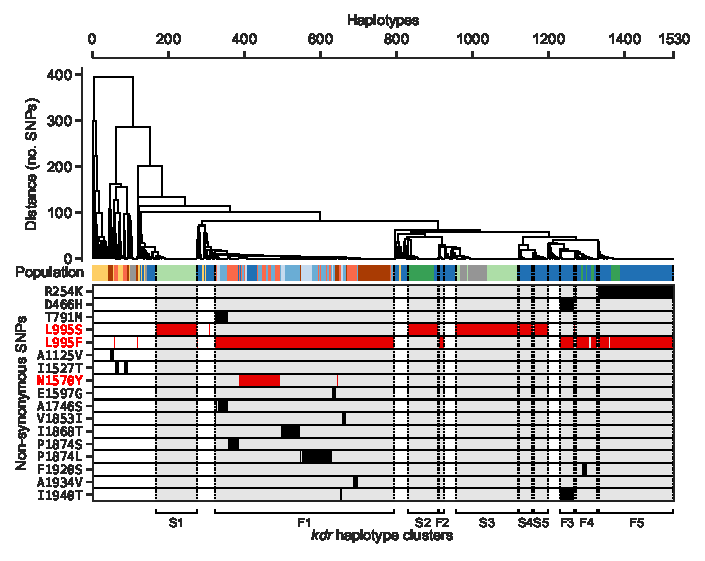
\includegraphics[width=\linewidth]{artwork/vgsc_haplotypes.pdf}
  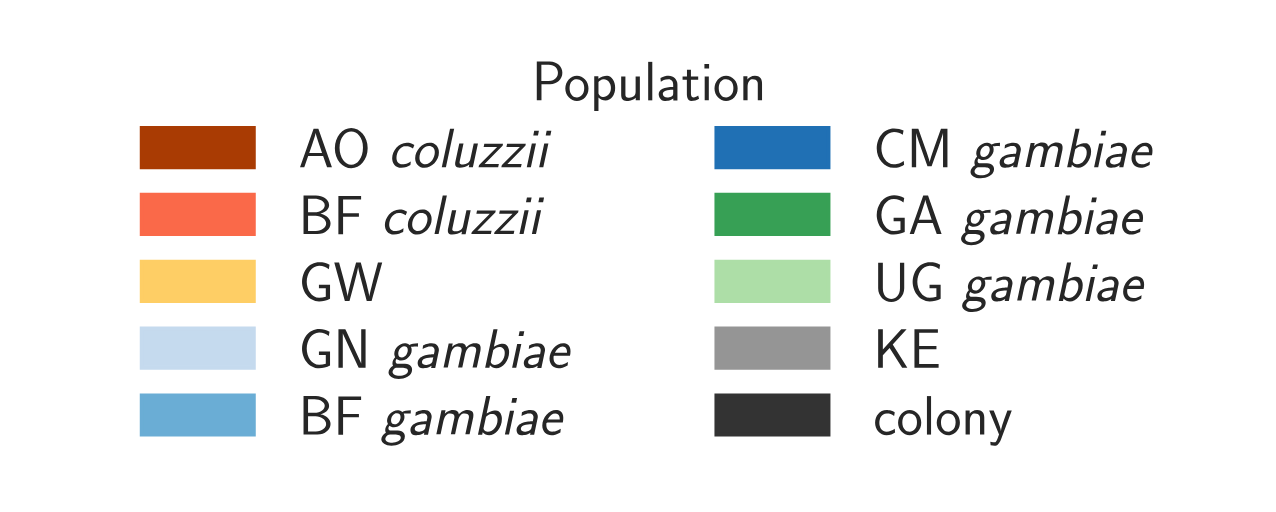
\includegraphics[width=0.5\linewidth]{artwork/pop_legend.png}

  \caption{\textbf{Hierarchical clustering of \vgsc haplotypes}. @@TODO caption.}

  \label{fig:vgsc_haplotypes}

\end{figure}
%%


%% describe hierarchical clustering
Figure \ref{fig:vgsc_haplotypes} shows a hierarchical clustering of the 1530 haplotype sequences derived from the 765 wild-caught mosquitoes.
%
This clustering was performed using variation data from within the full @@X kbp span of the \vgsc gene, which includes a total of @@N biallelic SNPs, of which @@M were synonymous and @@O were non-synonymous. 
%
The likely presence of recombination events within this genomic interval means that this clustering cannot be interpreted as a phylogeny, but rather as a descriptive analysis of genetic similarity.
%
However, it is clear from this analysis that there are several large clusters of near-identical haplotypes, each of which is strongly linked to one of the two \textit{kdr} alleles.
%
To provide a means of navigating these data, I cut the dendrogram at a maximum distance of @@N SNPs.
%
I then labelled the resulting clusters within which one of the two \textit{kdr} alleles was found (clusters F1-F5 carry the \texttt{L995F} allele, and clusters S1-S5 carry \texttt{L995S}).
%
These ten clusters accounted for @@X\% of haplotypes carrying a \textit{kdr} allele.
%%


%% make some argument as to why all haplotypes within these clusters must share a recent common ancestor
%
Within each cluster, at least @@X\% of haplotype pairs were identical, at least @@Y\% of haplotype pairs had at most a single SNP difference, and average divergence between haplotypes was @@X-@@Y\% (Supplementary Table @@TODO).
%
By comparison, within similar-sized windows, the genome-wide average level of genetic diversity within populations is in the range @@X-@@Y\%, and the average level of divergence between populations is @@X-@@Y\% (Supplementary Table @@TODO).
%
This comparison highlights the unusually low diversity within these clusters, especially for the clusters comprising haplotypes from multiple populations.
%
%%


%% describe patterns of geography and species in relation to clusters, and what this means for gene flow
%
Figure \ref{fig:vgsc_haplotypes} also provides a colour band that shows the country of origin and species of each mosquito from which each haplotype was derived.
%
@@TODO
%%


%%%%%%%%%%%%%%%%%%%%%%%%%%%%%%%%%%%%%%%%%%%%%%%%%%%%%%%%%%%%%%%%%%%%%%%%%%%%%%%
%%%%%%%%%%%%%%%%%%%%%%%%%%%%%%%%%%%%%%%%%%%%%%%%%%%%%%%%%%%%%%%%%%%%%%%%%%%%%%%
\section*{Discussion}


%%%%%%%%%%%%%%%%%%%%%%%%%%%%%%%%%%%%%%%%%%%%%%%%%%%%%%%%%%%%%%%%%%%%%%%%%%%%%%%
\subsection*{TODO}


%%
TODO
%%


%%%%%%%%%%%%%%%%%%%%%%%%%%%%%%%%%%%%%%%%%%%%%%%%%%%%%%%%%%%%%%%%%%%%%%%%%%%%%%%
%%%%%%%%%%%%%%%%%%%%%%%%%%%%%%%%%%%%%%%%%%%%%%%%%%%%%%%%%%%%%%%%%%%%%%%%%%%%%%%
\section*{Methods}


%%%%%%%%%%%%%%%%%%%%%%%%%%%%%%%%%%%%%%%%%%%%%%%%%%%%%%%%%%%%%%%%%%%%%%%%%%%%%%%
\subsection*{TODO}

%%
TODO
%%


%%%%%%%%%%%%%%%%%%%%%%%%%%%%%%%%%%%%%%%%%%%%%%%%%%%%%%%%%%%%%%%%%%%%%%%%%%%%%%%
%%%%%%%%%%%%%%%%%%%%%%%%%%%%%%%%%%%%%%%%%%%%%%%%%%%%%%%%%%%%%%%%%%%%%%%%%%%%%%%
\printbibliography


%%%%%%%%%%%%%%%%%%%%%%%%%%%%%%%%%%%%%%%%%%%%%%%%%%%%%%%%%%%%%%%%%%%%%%%%%%%%%%%
%%%%%%%%%%%%%%%%%%%%%%%%%%%%%%%%%%%%%%%%%%%%%%%%%%%%%%%%%%%%%%%%%%%%%%%%%%%%%%%
%%%%%%%%%%%%%%%%%%%%%%%%%%%%%%%%%%%%%%%%%%%%%%%%%%%%%%%%%%%%%%%%%%%%%%%%%%%%%%%
\beginsupplement
\clearpage


%%%%%%%%%%%%%%%%%%%%%%%%%%%%%%%%%%%%%%%%%%%%%%%%%%%%%%%%%%%%%%%%%%%%%%%%%%%%%%%
%%%%%%%%%%%%%%%%%%%%%%%%%%%%%%%%%%%%%%%%%%%%%%%%%%%%%%%%%%%%%%%%%%%%%%%%%%%%%%%
\section*{Supplementary figures}


%% Figure - VGSC accessibility.
%
\afterpage{%
\newgeometry{margin=2cm}
\begin{landscape}
\thispagestyle{empty}

\begin{figure}[!t]

  \centering

  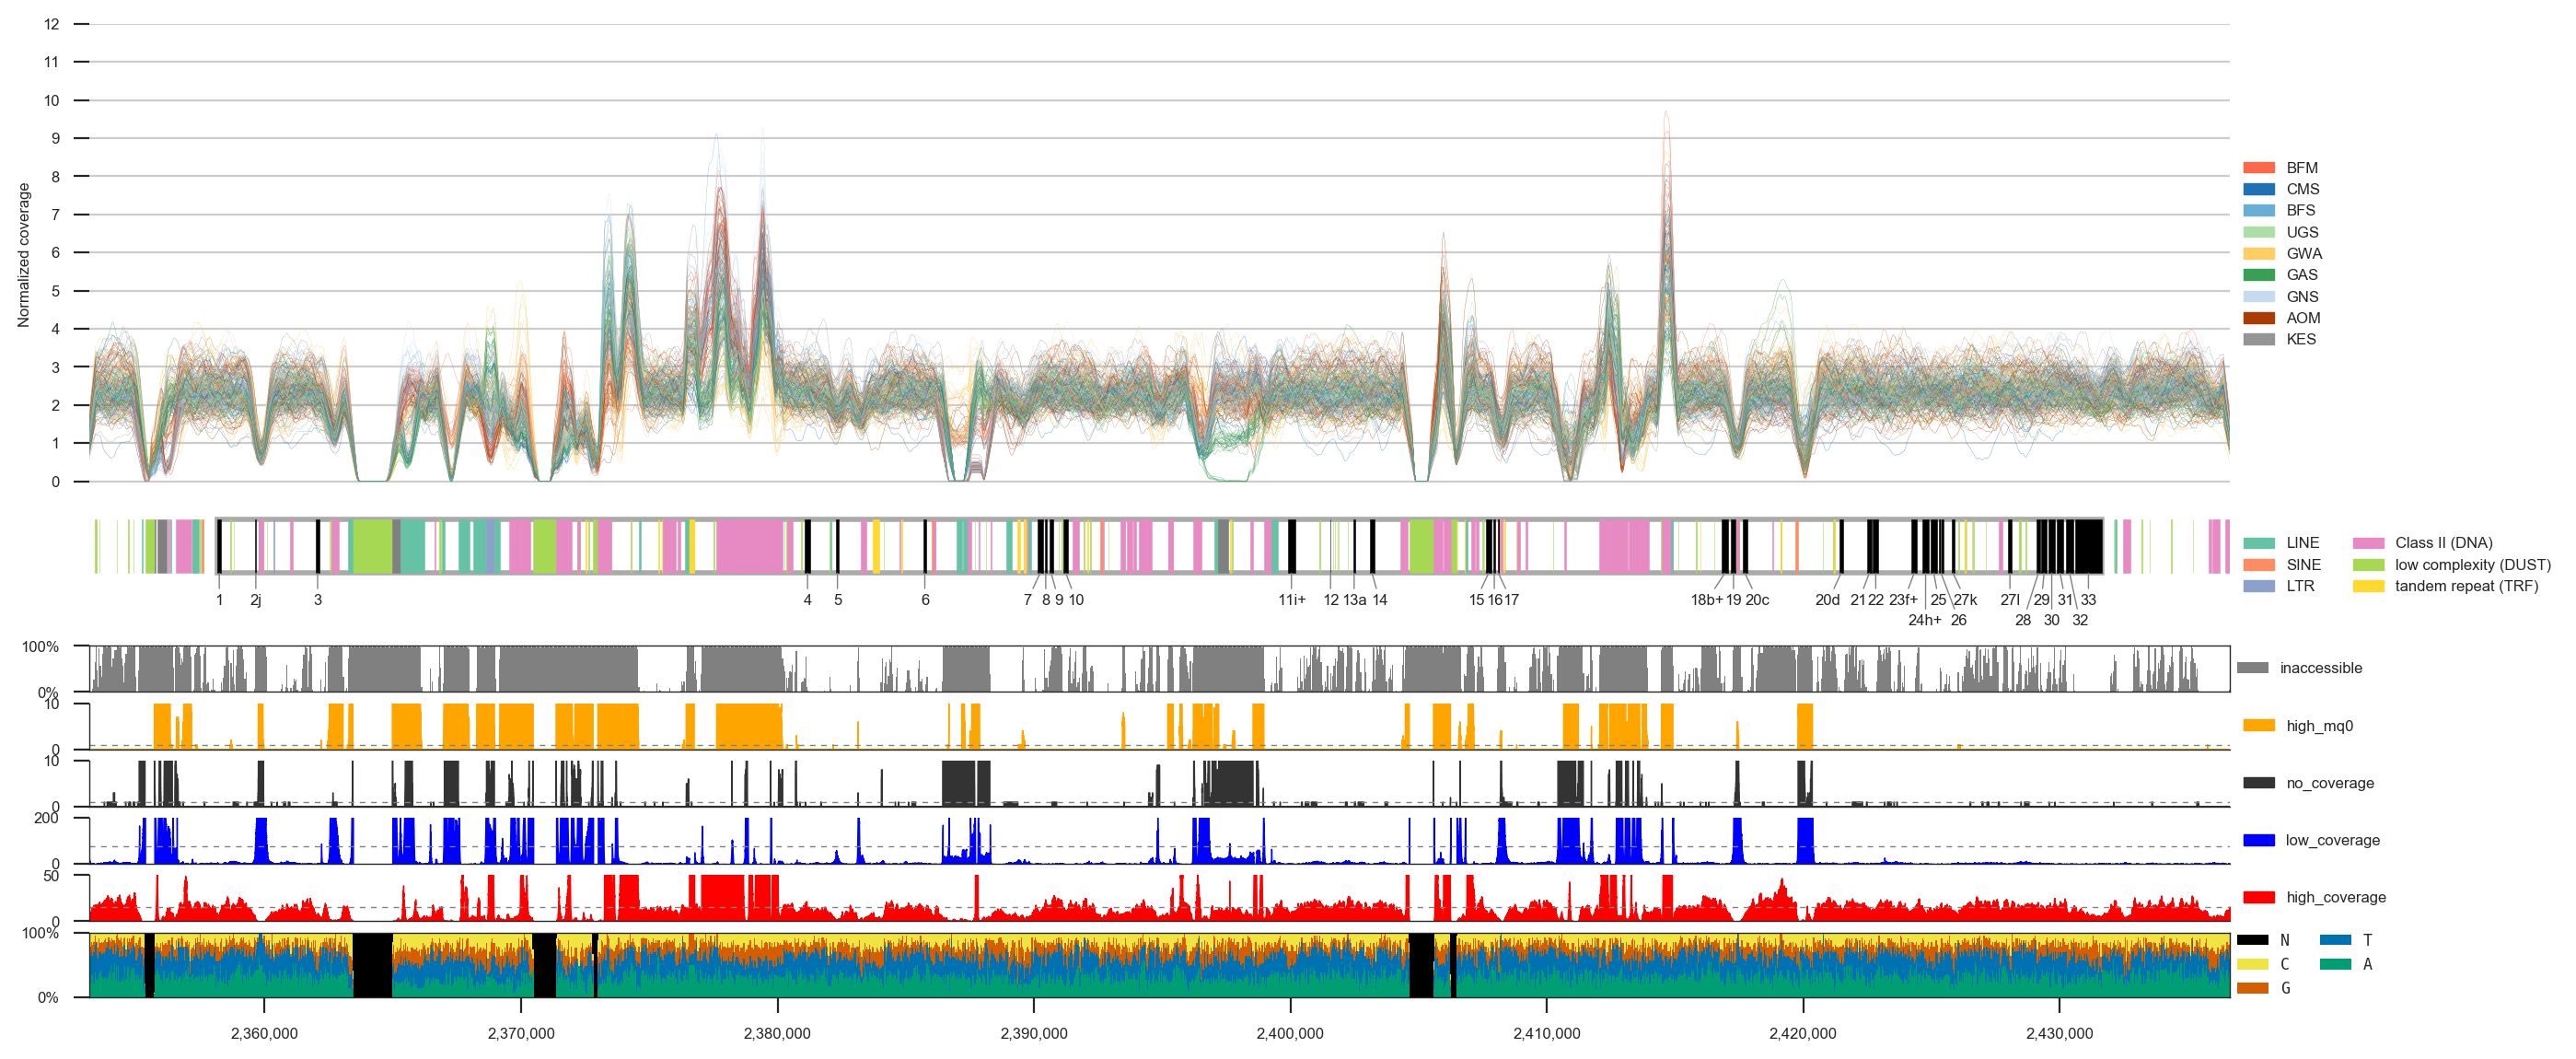
\includegraphics[width=\linewidth]{artwork/vgsc_accessibility_overview.png}

  \caption{\textbf{Accessibility of the \vgsc gene}. @@TODO caption.}

  \label{fig:accessibility}

\end{figure}
%%

\end{landscape}
\restoregeometry
} % end afterpage
%% end Figure


%% Figure - VGSC transcripts.
%
\afterpage{%
\newgeometry{margin=2cm}
\begin{landscape}
\thispagestyle{empty}

\begin{figure}[!t]

  \centering

  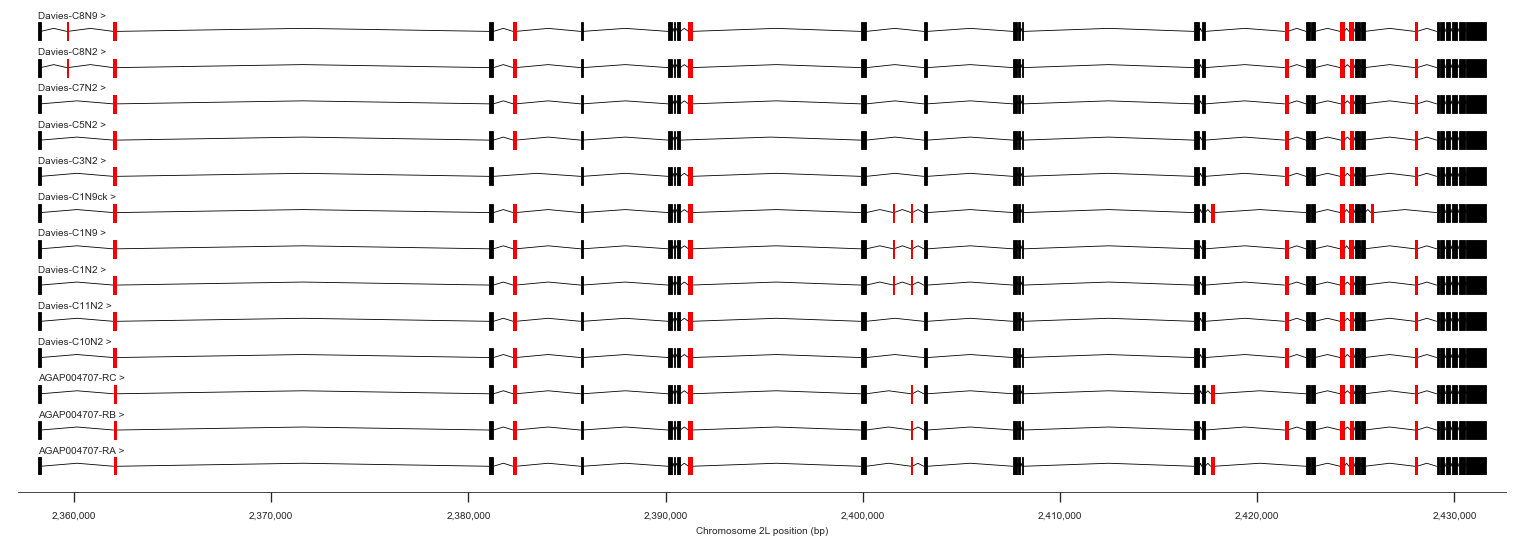
\includegraphics[width=\linewidth]{artwork/vgsc_transcripts.png}

  \caption{\textbf{\vgsc transcripts}. @@TODO caption.}

  \label{fig:transcripts}

\end{figure}
%%

\end{landscape}
\restoregeometry
} % end afterpage
%% end Figure


\clearpage


%%%%%%%%%%%%%%%%%%%%%%%%%%%%%%%%%%%%%%%%%%%%%%%%%%%%%%%%%%%%%%%%%%%%%%%%%%%%%%%
%%%%%%%%%%%%%%%%%%%%%%%%%%%%%%%%%%%%%%%%%%%%%%%%%%%%%%%%%%%%%%%%%%%%%%%%%%%%%%%
\section*{Supplementary tables}


\end{document}
